\documentclass[12pt]{article}
\usepackage[utf8]{inputenc}
\usepackage{pgfplots}

\title{Python Programming MMO}
\author{Sol Steele}
\date{July 2018}


\setlength{\parindent}{1em}
\setlength{\parskip}{1em}
\setlength{\parindent}{0em}

\usepackage[a4paper, margin=1in]{geometry}


\usepackage[utf8]{inputenc}
\usepackage{graphicx}
\usepackage{minted}
\usepackage{natbib}
\usepackage{graphicx}
\usepackage{listings}
\usepackage{pythonhighlight}
\usepackage{dirtree}
\usepackage{tikz}
\usetikzlibrary{positioning}
\usepackage{lscape}
\usepackage{listings}
\usepackage{color}
\usepackage{mdframed}
\usepackage{placeins}

\def\code#1{\texttt{#1}}

\definecolor{codegreen}{rgb}{0,0.6,0}
\definecolor{codegray}{rgb}{0.5,0.5,0.5}
\definecolor{codepurple}{rgb}{0.58,0,0.82}
\definecolor{backcolour}{rgb}{0.95,0.95,0.92}

\lstdefinestyle{mystyle}{
    backgroundcolor=\color{backcolour},   
    commentstyle=\color{codegreen},
    keywordstyle=\color{magenta},
    numberstyle=\tiny\color{codegray},
    stringstyle=\color{codepurple},
    basicstyle=\footnotesize,
    breakatwhitespace=false,         
    breaklines=true,                 
    captionpos=b,                    
    keepspaces=true,                 
    numbers=left,                    
    numbersep=5pt,                  
    showspaces=false,                
    showstringspaces=false,
    showtabs=false,                  
    tabsize=2
}

\definecolor{lightgray}{rgb}{.9,.9,.9}
\definecolor{darkgray}{rgb}{.4,.4,.4}
\definecolor{purple}{rgb}{0.65, 0.12, 0.82}

\lstdefinelanguage{JavaScript}{
  keywords={typeof, new, true, false, catch, function, return, null, catch, switch, var, if, in, while, do, else, case, break},
  keywordstyle=\color{blue}\bfseries,
  ndkeywords={class, export, boolean, throw, implements, import, this},
  ndkeywordstyle=\color{darkgray}\bfseries,
  identifierstyle=\color{black},
  sensitive=false,
  comment=[l]{//},
  morecomment=[s]{/*}{*/},
  commentstyle=\color{purple}\ttfamily,
  stringstyle=\color{red}\ttfamily,
  morestring=[b]',
  morestring=[b]"
}

\lstset{
   language=JavaScript,
   backgroundcolor=\color{lightgray},
   extendedchars=true,
   basicstyle=\footnotesize\ttfamily,
   showstringspaces=false,
   showspaces=false,
   numbers=left,
   numberstyle=\footnotesize,
   numbersep=9pt,
   tabsize=2,
   breaklines=true,
   showtabs=false,
   captionpos=b
}
 
\lstset{style=mystyle}


\pgfplotsset{compat=1.15}

\begin{document}

\begin{titlepage}
    \centering
    \begin{center}
        
\includegraphics[width=10cm]{ThsLogo.png}
    \end{center}
    {\scshape\LARGE The Thomas Hardye School\par}
{\scshape\Large Computer Science Project\par}
\vspace{1.5cm}
{\huge\bfseries Python Programming MMO\par}
\vspace{0.5cm}
{\Large\itshape \textbf{Sol Steele}\par}
{\Large\itshape Candidate number: \#\#\#\#\par}
{\Large\itshape Center number: 55321\par}
\vfill
{\large \today\par}
\end{titlepage}

\tableofcontents
\newpage

\section{Analysis}
\subsection{Problem Identification}
There are already quite a few games for teaching younger people programming but they fail to keep the users engaged for any long period of time. A game to teach programming while retaining entertaining would provide many benefits for teachers and students alike. It would provide and environment where they can try and experiment with code while seeing the code have an effect in the game world. Often in this environment students want to show off their code to friends or the teacher see what they are doing.

The game would be a massively multiplayer online game (MMO), this means that all the users connect to a central server and are all on the same world and working together or against each other.

To allow it to be used more easily by schools and programmers I would have it run in browser with JavaScript web sockets and HTML5 canvases. This means that the project would have very good cross platform support and it is operating system independent.

This is a good problem to be solved computational as it would be teaching computational thinking. This means that the program must have a good understanding of computational thinking to be able to teach it.

\subsection{Stake Holders}
The demographic of my project will be students learning the beginning of code, people who want to reinforce the basics and improve their code and teachers wanting an interactive way to engage students with programming. 

It would be useful for students as it would have tutorial for programming in the language the game uses and it would be able to learn the code in an active environment and see its effects on the environment. Having a way to see what there code does and having a moving end goal will be motivation for them to improve the programming skills and share their creation.

It would also be useful for teachers as they will be able to monitor and give advice on the students’ code. This would allow, not only the internal tutorial in the game, but also an actual teacher in a school environment.

The game could also be good for teaching co-operation and how to work on a group project in programming as you can have a large amount of code written by different people all functioning in tandem to meet a goal

\subsection{Why is it suited to a computational solution}
The problem is directly linked to a computational solution because teaching people how to write a program would need the program to be run. This would require a computer to operate. The rendering of complex graphics for the user’s interaction with the game would need to run on a computer as it will be directly affected by a central server. It all needs to be done in an environment where network communication can be quick.

\subsection{Computation methods that would be used}
\subsubsection{Problem Recognition}
The main problem to be solved is how to store and render the world that the users would be interacting with and running the user submitted code to control the characters in the world. Once this has been broken down into smaller problems the implementation of each small part should not be too complex. My main difficulty in the project would be the server security as it would have programs written by users running on it and these may have malicious intent, so I need to control what the user can do without limiting their ability to learn programming.

\subsection{Problem Decomposition}
The program can be broken down into 3 main section each can be broken down even further.

\subsubsection{Server}
This is the main overarching decomposition but each section will need to be broken down further
\begin{itemize}
    \item The server that the users will talk to
    \item The WebApp that will be used by the users for talking to the server
    \item A server control system and website for setting up accounts
\end{itemize}
Even with the decomposition into the smaller steps and function each one can be made into even smaller function, this would make the program easier to code and maintain, this would make a more readable code sample and future upgradability.

\subsubsection{WebApp}
This is what the user will be using to interact with the server, it will need to be intuitive and functional. The faster this can run the more accessible it is as it will run on older computers.
It will need many functions such as:
\begin{itemize}
    \item Displaying the UI and the world around the player
    \item Taking user input, such as panning the screen or submitting code.
    \item Communication with the server
\end{itemize}
This would be the main part of the program that the user will see.

\subsubsection{Website/System Control}
This would be mainly for account creation and user verification, it should also have an admin mode for server monitoring. The problem could be broken down like this:
\begin{itemize}
    \item The main HTML and CSS for displaying the site to the user
    \item Some networking to the server and a database to manage user accounts
    \item Server and network usage monitoring.
\end{itemize}

\newpage
\subsection{Interview}
For an interview I set up a survey on the website www.surveymonkey.com. This site allows you to make a survey and have people answer it online. I shared the survey on a programming community at www.devrant.com as they represent a large section of my stakeholder demographic. In total I got 9 results.


\subsubsection{Questions:}
\textbf{Question 1}

"What is your relationship with programming?"
2 people say they are avid and experienced programmers.
the other 7 say they can program enough for what they need.

This means that the people who did the survey do not fill out the section for teaching people how to program. But the data will still be useful for people who may want to improve there skill but not start from the beginning.


\textbf{Question 2}

"Did you use an application or program to learn programming? (Such as Codecademy or Hour of Code)"
7 people responded yes and 2 people responded no.

This shows that lots of people have used online educational tools to learn programming. Although the people who responded to my survey say they all ready know how to code this question shows me one of the ways they learns how.

There was a follow up question to ask if they would recommend it to someone learning programming.

All responses were anonymous:

"It was fun but not really helpful"\newline
"Not really. Docs are way more structured."\newline
"I would recommend this as it walks you though the syntax of a language and it goes at a pace you are comfortable leaning at"\newline
"Yes as it teaches u in steps"\newline
"Hour of code is really basic but good for fundamental knowledge, and its quite fun - so I would recommend it to someone who hasn't done any programming before."\newline
"I would recommend something like this as it can walk you through the process of understanding the syntax of a language from the basics to the more advanced at a pace you are comfortable with"\newline
"No, they're all bad. It's better to learn from documentation and websites like tutorialspoint"

So from these responses 5 people would recommend it as a useful tool for learning. and the other 2 find that learning from the raw documentation is better/more structured.


\textbf{Question 3}

"Have you played any educational games to teach programming? (Such as TIS100 or The Human resource machine)"
3 people responded yes and 6 responded no.

I found this surprising due to the large emergence of programming games in recent years, but it could be explained by the fact that a lot of the games are aimed for younger audiences.

This was again follow up question to see if they would recommend it to people learning programming. There were only 2 responses.

"Yes indeed HRM is lit" 

"Yes. I played The Human Resource Machine and it doesn't really help with learning programming, but it's fun "

The responses seem to only recommend the game for its entertainment value and not as a tool for teaching programming.


\textbf{Question 4}

This question is asking how they first learnt how to program. There were 7 options that the person could agree with. They could tick as many boxes as they like.

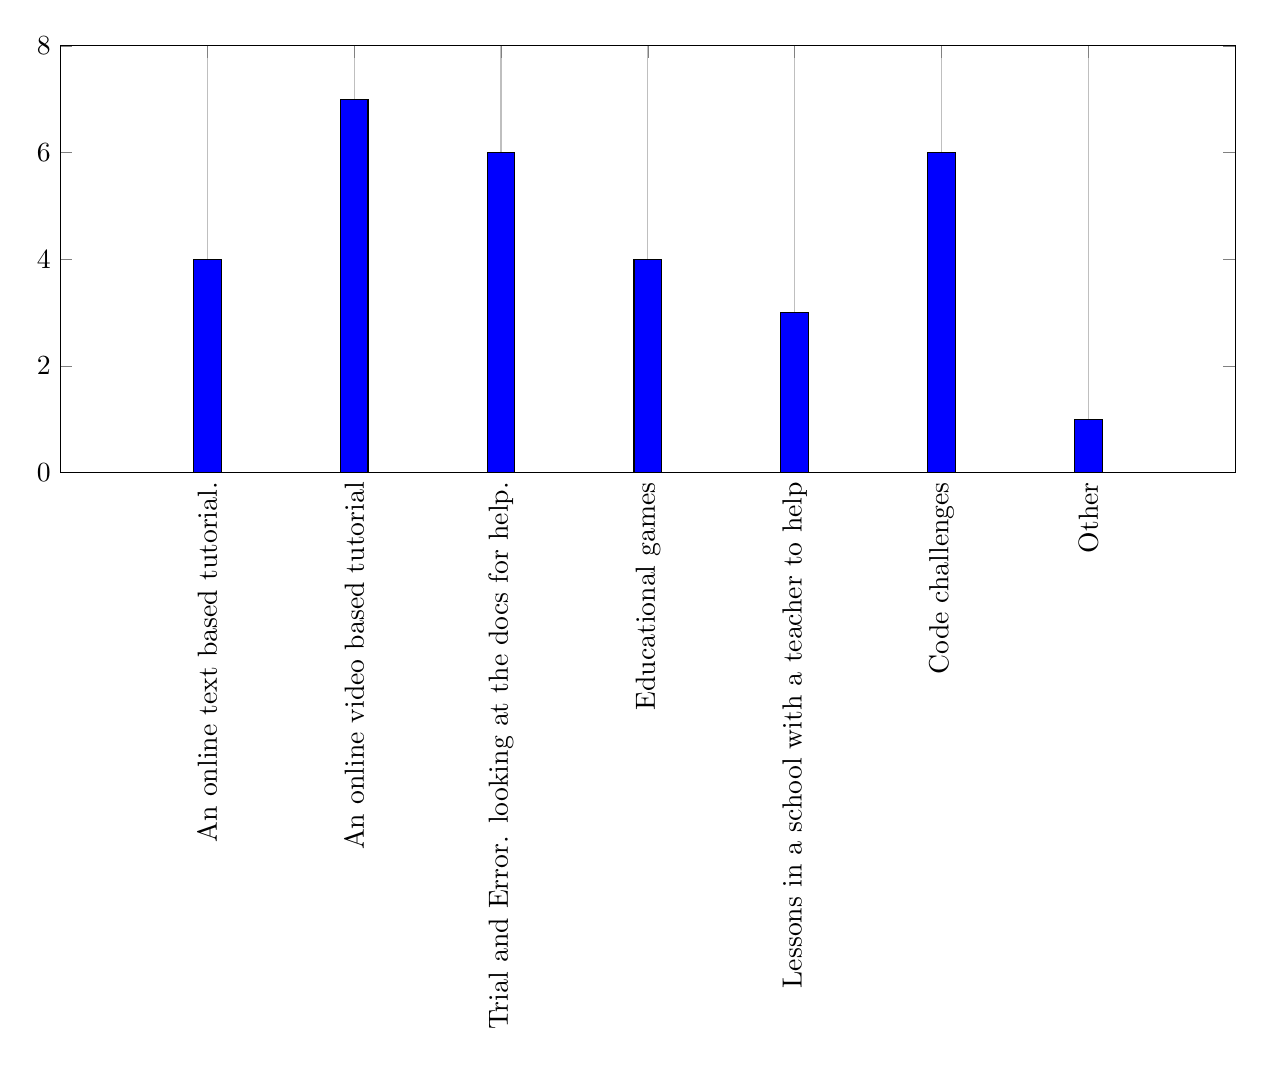
\begin{tikzpicture}
\begin{axis}[
    width=16.5cm,
    height=7cm,
    xmin=-1 ,xmax=7,
    ymin=0, ymax=8,
    xtick=\empty,
    extra x ticks={0,1,2,3,4,5,6},
    extra x tick labels={
        An online text based tutorial., 
        An online video based tutorial, 
        Trial and Error. looking at the docs for help., 
        Educational games, 
        Lessons in a school with a teacher to help, 
        Code challenges, 
        Other, 
        },
    extra x tick style={
           grid=major,
           tick label style={rotate=90}
           }
    ]
    \addplot[ybar, fill=blue] coordinates{(0,4)};
    \addplot[ybar, fill=blue] coordinates{(1,7)};
    \addplot[ybar, fill=blue] coordinates{(2,6)};
    \addplot[ybar, fill=blue] coordinates{(3,4)};
    \addplot[ybar, fill=blue] coordinates{(4,3)};
    \addplot[ybar, fill=blue] coordinates{(5,6)};
    \addplot[ybar, fill=blue] coordinates{(6,1)};

\end{axis}
\end{tikzpicture}

The one person who said other put "A combination of text and video would be helpful (a link to a doc)"

This question's responses show that the people learnt programming from mainly non interactive sources. With most people saying Online video tutorials. The second biggest one was just hands on work with the code, represented by code challenges and Trial and Error. Only a third of people who answered the questions had taken lessons in programming.


\textbf{Question 5}

"Would you play an online competitive/cooperative programming game?"

This was on a scale.\newline
"I would play it for fun"\newline
"Only if a teacher made me"\newline
"I might try it"\newline
"Never"

All 9 people responded with "I would play it for fun."

This shows that in the demographic of the survey there is a large demand for this type of game.


\textbf{Question 6}

"What language(s) would you want such a game to support?"

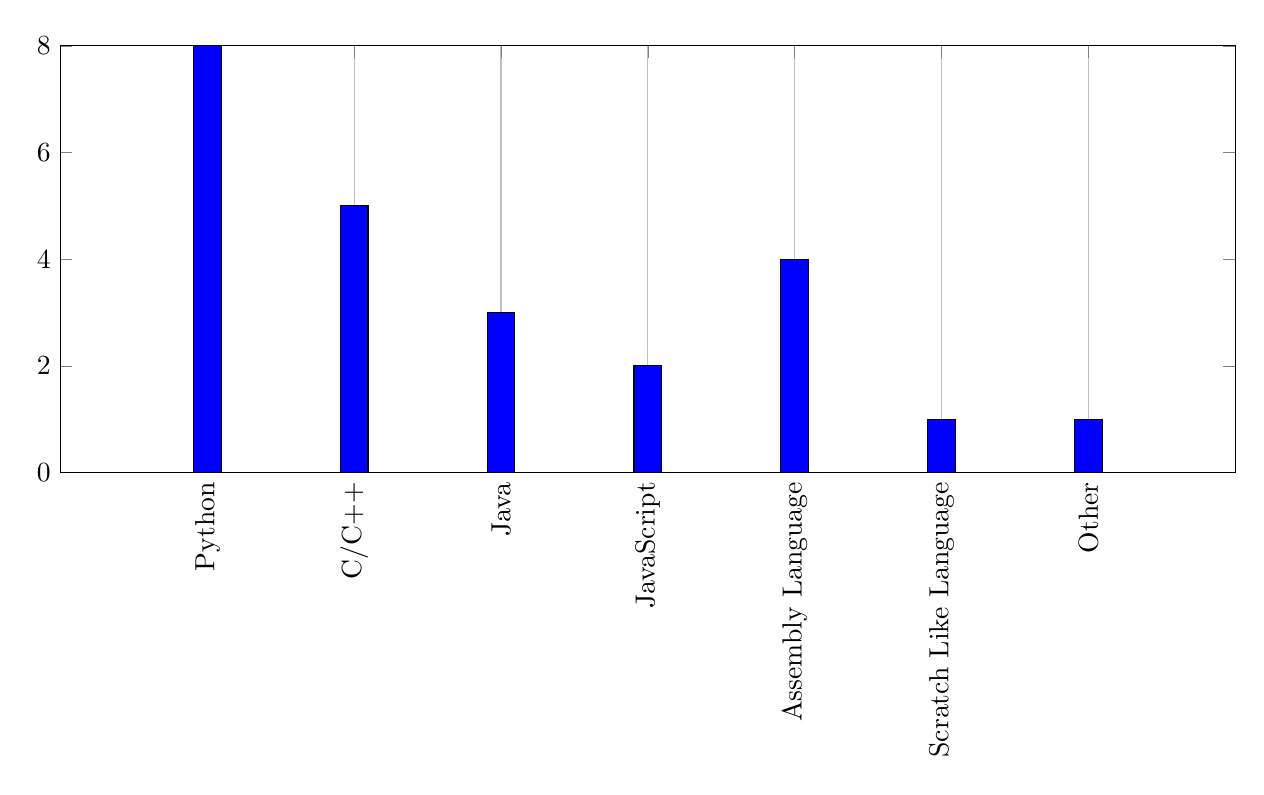
\begin{tikzpicture}
\begin{axis}[
    width=16.5cm,
    height=7cm,
    xmin=-1 ,xmax=7,
    ymin=0, ymax=8,
    xtick=\empty,
    extra x ticks={0,1,2,3,4,5,6},
    extra x tick labels={
        Python,
        C/C++,
        Java,
        JavaScript,
        Assembly Language,
        Scratch Like Language,
        Other,
        },
    extra x tick style={
           grid=major,
           tick label style={rotate=90}
           }
    ]
    \addplot[ybar, fill=blue] coordinates{(0,8)};
    \addplot[ybar, fill=blue] coordinates{(1,5)};
    \addplot[ybar, fill=blue] coordinates{(2,3)};
    \addplot[ybar, fill=blue] coordinates{(3,2)};
    \addplot[ybar, fill=blue] coordinates{(4,4)};
    \addplot[ybar, fill=blue] coordinates{(5,1)};
    \addplot[ybar, fill=blue] coordinates{(6,1)};

\end{axis}
\end{tikzpicture}

The "Other" response wanted to include the language Go

While possible to include all the requested languages into the program due to the score of the task I will only plan on incorporating a simple language such as Python or C/C++.


\subsubsection{Analysis}
The questionnaire only gives me data on people who already know quite a bit of programming. The response on the use of games and interactive media for learning programming is quite different to what I expected. The main response was that the people learnt programming by trying it out and watching video tutorials. With this data I think that it will be necessary to make the game have a lose tutorial on some concepts but leave most of the learning up to the user. The large amount of people who say they learnt from code challenges leads me to think that while a self motivated learning environment would be useful it could also be good if I provide a set of clearly set out goals to drive there ability forward while not limiting the method to get there.


\newpage
\subsection{Research}
\subsubsection{Existing similar solutions}

\textbf{Games:}

\texttt{\textbf{Screeps>\_}}\newline
Overview:\newline
Screeps>\_ is a game where many users are on the same map. It is user programmed in JavaScript. In the game people compete for a resources. They are used to produce things that the user needs to expand. There are 7 key resources that are used in a series of more and more complex reactions to produce the final product. This is quite a popular game with a 8.9/10 score on the site Steam (www.steampowered.com). There is a large community of people in the game that create a thriving interactive world.

{\centering
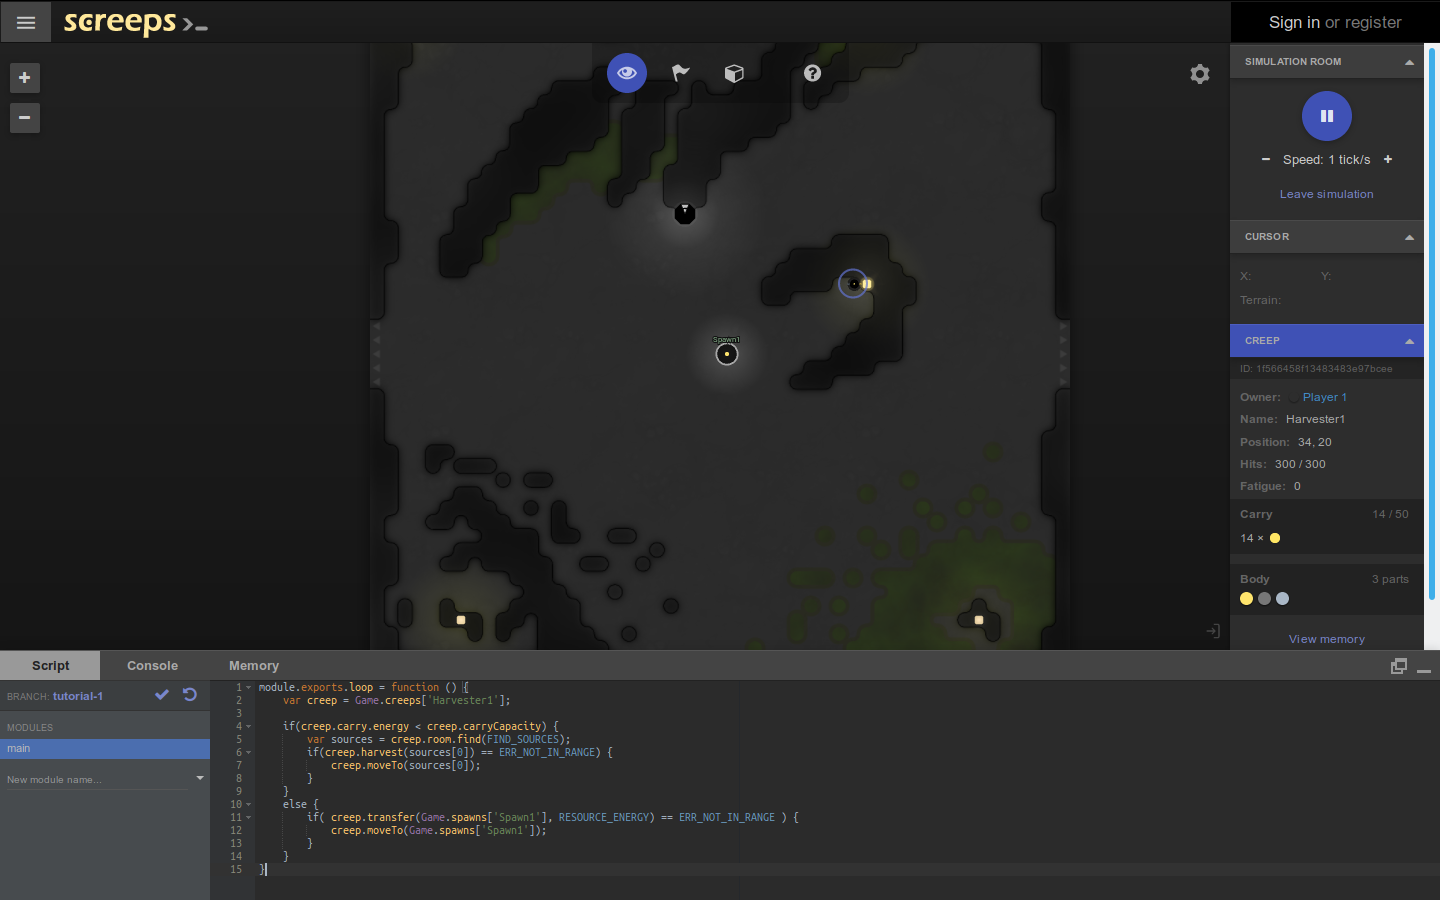
\includegraphics[width=15cm]{Images/screeps.png}\par
}

The screen shot is from the tutorial of the game. One major flaw of the game is that it is unfriendly to new players. Its interactive tutorial dumps you in the deep end and just gives you code snippets to learn from. It doesn't give you much direction on what the code does and just refers you to the documentation for the project. This could be useful for people playing it for the game but it could be quite daunting for people playing to just start programming.


What can I take from this?:\newline
From my short time testing the game I can see that it is important to have a simple and approachable tutorial for new players but also not limit the learning of the game to the tutorial. It is important to allow people of all skill levels to enjoy. 
The multiplier aspect of the game keeps the users attention and has them keep coming back to the game. This is impotent if I am going to use this to teach programming as spaced learning is necessary to reinforce skills.
The game also has a useful API which allows people to create there own programs to talk to the server. This is used by a lot of people as if they are unhappy with the IDE the game provides they can very easily set up there own.


\textbf{Human Resource Machine}\newline
Overview:\newline
The game published by Tomorrow Corporation
This is a game where you control an office worker who faces a job environment of increasing automation. The game is programmed with a visual assembly like programming language. This is a fun game that has seen very positive reviews getting a 9.4/10 on Steam (www.steampowered.com). The game is not very good at teaching modern programming though. The programme flow relies heavily on jumps and conditional jumps. This is not the best for teaching programming but it is a good way to teach computational thinking.

{\centering
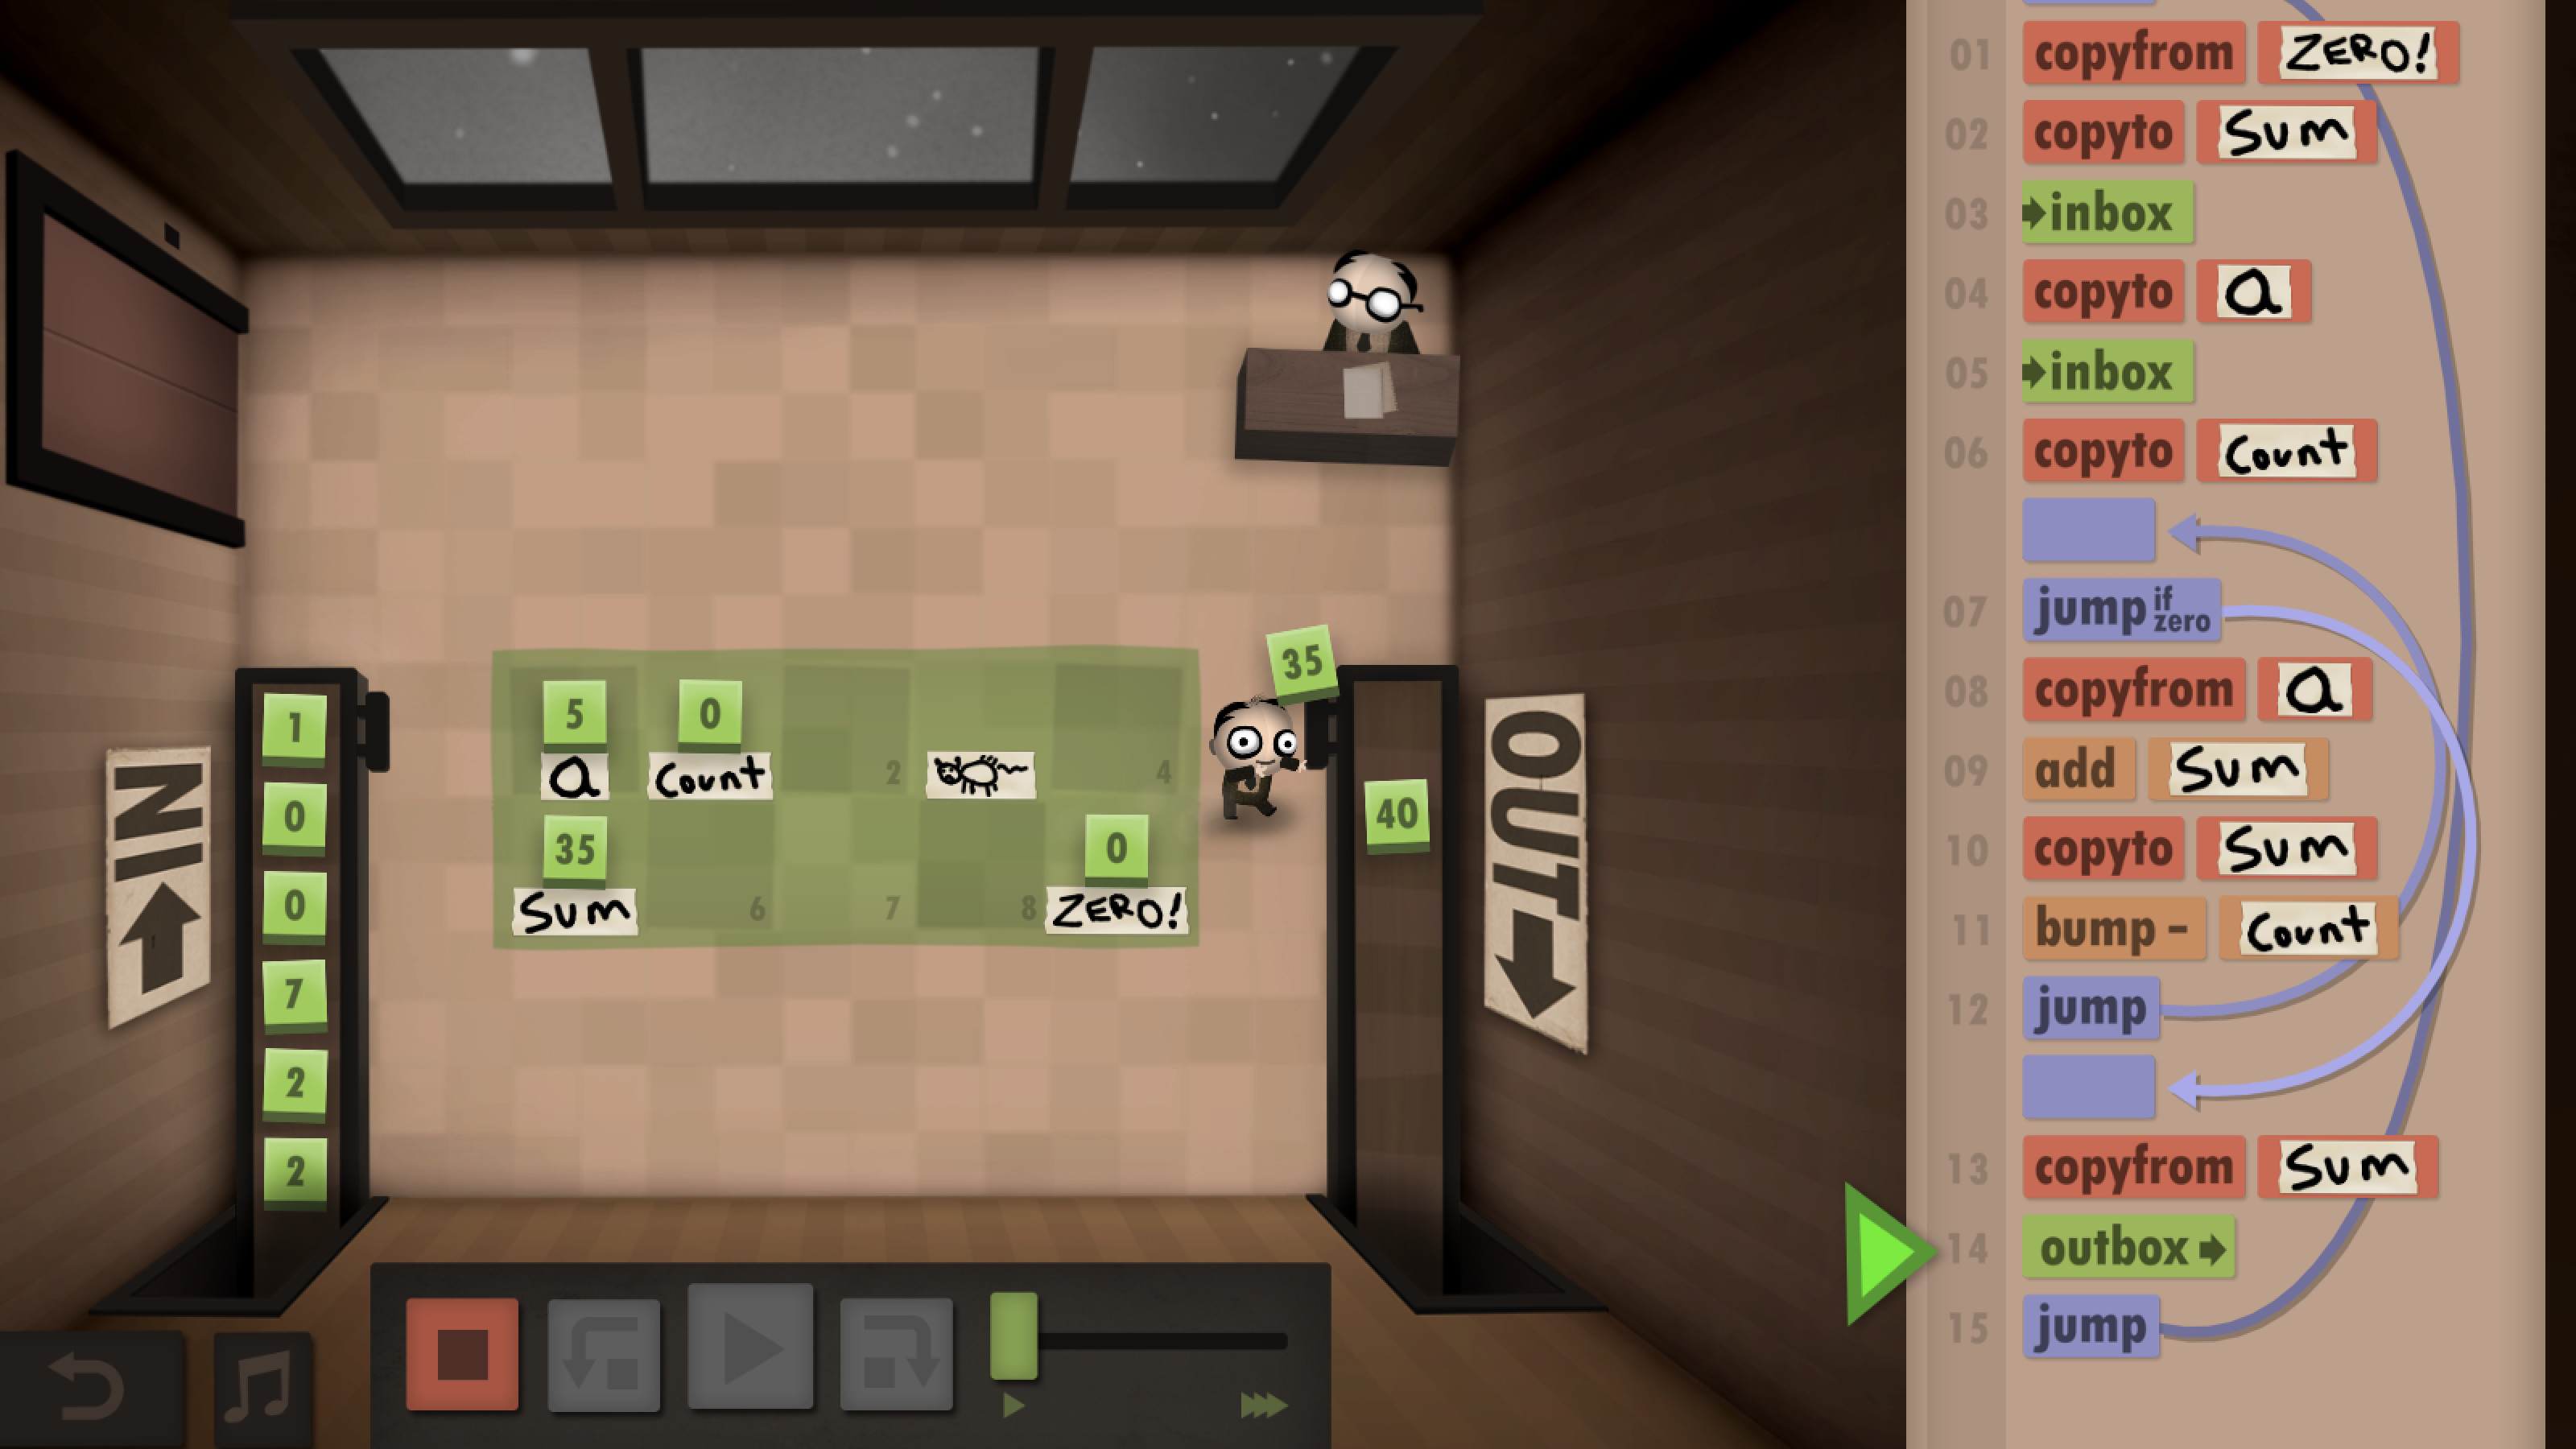
\includegraphics[width=15cm]{Images/HumanResourceMachine.jpg}\par
}

The art of the game and over all style are very charming and provide for a fun and educational time.

What can I take from this?:\newline
What the game shows is that with an attractive art style and charming story you can grab a wide audience by showing it as a puzzle game. This is shown by the much wider reception of the game and even a mobile release.

\textbf{7 Billion Humans}\newline
Overview:\newline
This game is a direct sequel to Human Resource Machine by Tomorrow Corporation. It is a very similar concept but it uses swarms of people instead of one. This means that you have to write multithread-able code that can be run concurrently on masses of operators.

{\centering
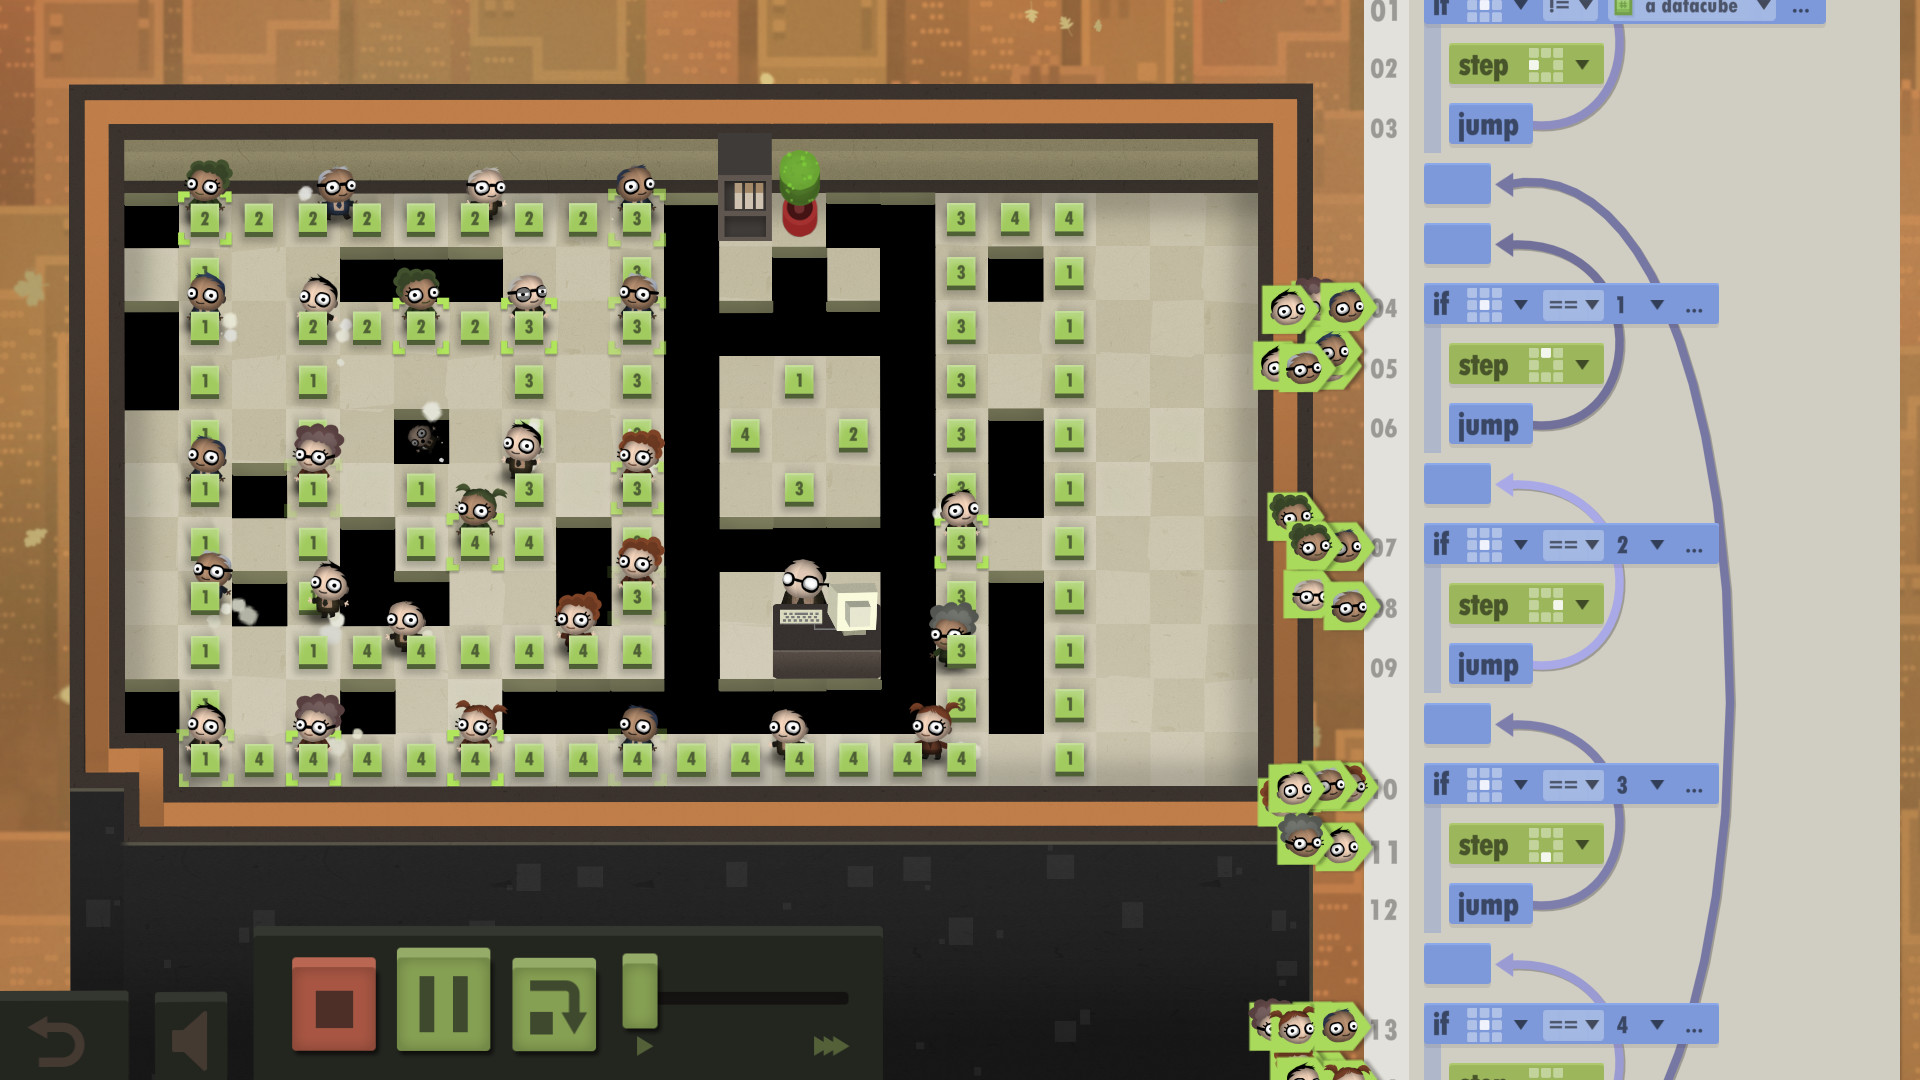
\includegraphics[width=15cm]{Images/7Billion.jpg}\par
}

What can I take from this?:\newline
The fact that Human Resource Machine was successful enough to get a sequel shows that if presented to a wide audience the reception can be very good for what I thought was quite a niche game genre. But the limiting things that you can do with the scripting language that they give you can get quite frustrating when you have to do high level things in such a low level language.

\textbf{TIS-100}\newline
Overview:\newline
The game is presented with quite an odd programming language. The code its self is just a simple Assembly code but it is made up of 12 blocks. Each of which can be a code block or a stack block. Each code block can talk to input nodes and other blocks. This makes for some quite strange code where you have many sections of at most 15 lines of Assembly talking to each other. The game has quite a small reception and not much user retention. It is presented as more of a puzzle game for seasoned programmers than a way to learn programming.

{\centering
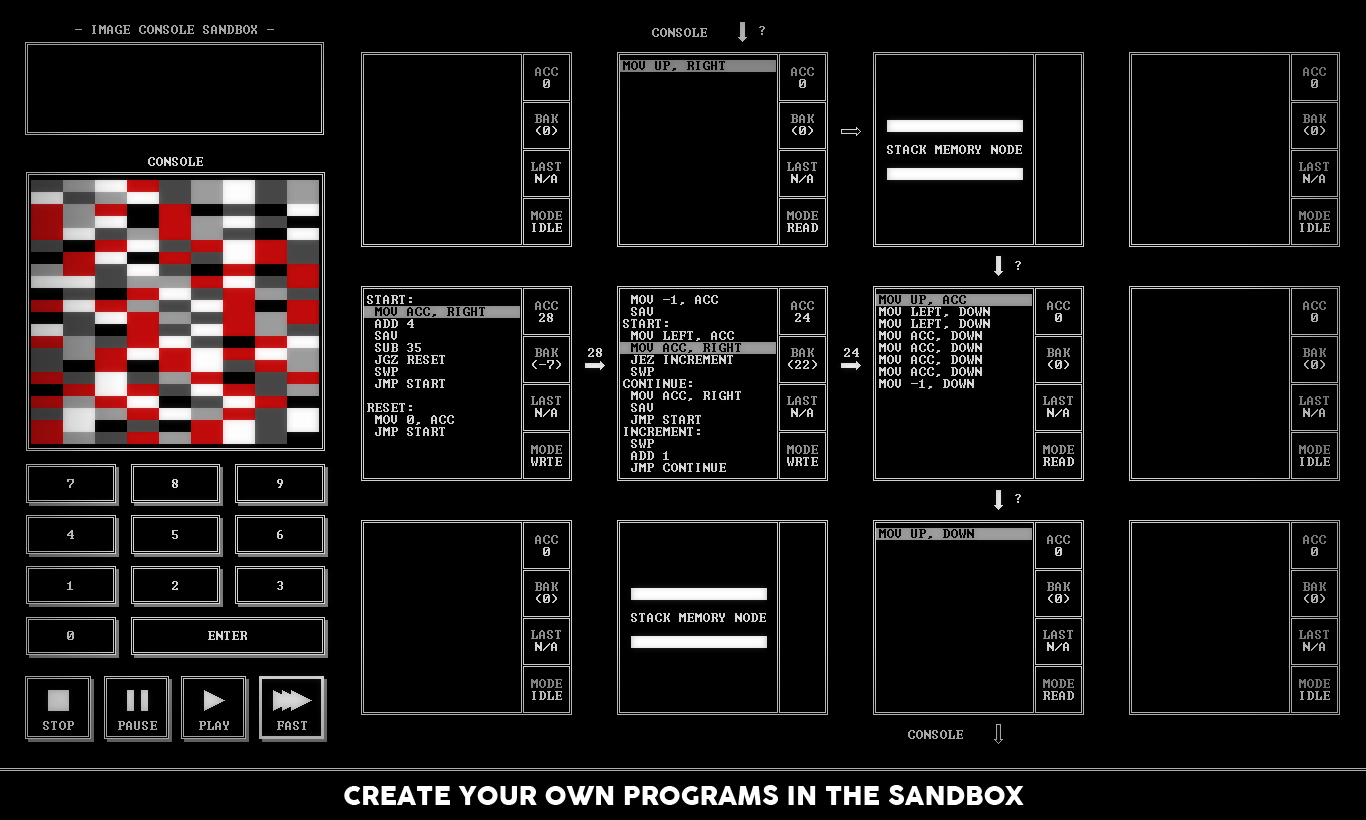
\includegraphics[width=15cm]{Images/tis-100.jpg}\par
}

What can I take from this?:\newline
This game, while very fun, provides not much educational use in learning programming and is much better at reinforcing the ideas of computation thinking and problem solving. It is quite good for entertainment and finding out how to approach a problem with coding as a solution but is not ideal for teaching them a useful language.

\textbf{Educational Tools:}

\textbf{CodeCademy}

{\centering

\includegraphics[width=8cm]{Images/codecademy_logo.png}\par
}
CodeCademy is a website aimed at teaching people programming among other skills. It is used in schools for programming as it has a build in IDE and programming environment allowing code to be run with out needing to install anything locally. It mainly has text tutorials, small demos and it checks if your code fulfils the challenge criteria it walks you through in small steps and has been quite successful for teaching programming. But looking at the survey I did this type of tool seems to be quite polarising as people ether think it is good for teaching programming or not useful at all. 

What can I take from this?:\newline
The integration into the browser has seen this program used in educational environments as it is easy to set up so for my project I would like to mirror this feature and have the user end of the game running completely in a browser.

\textbf{Hour of Code}\newline
Hour of code is based on a similar premise to CodeCademy but it is aimed at a younger audience and it has the backing of large companies such as Mojang and Disney so they can use popular Intellectual properties such as Minecraft or StarWars to try and engage the audience.
{\centering
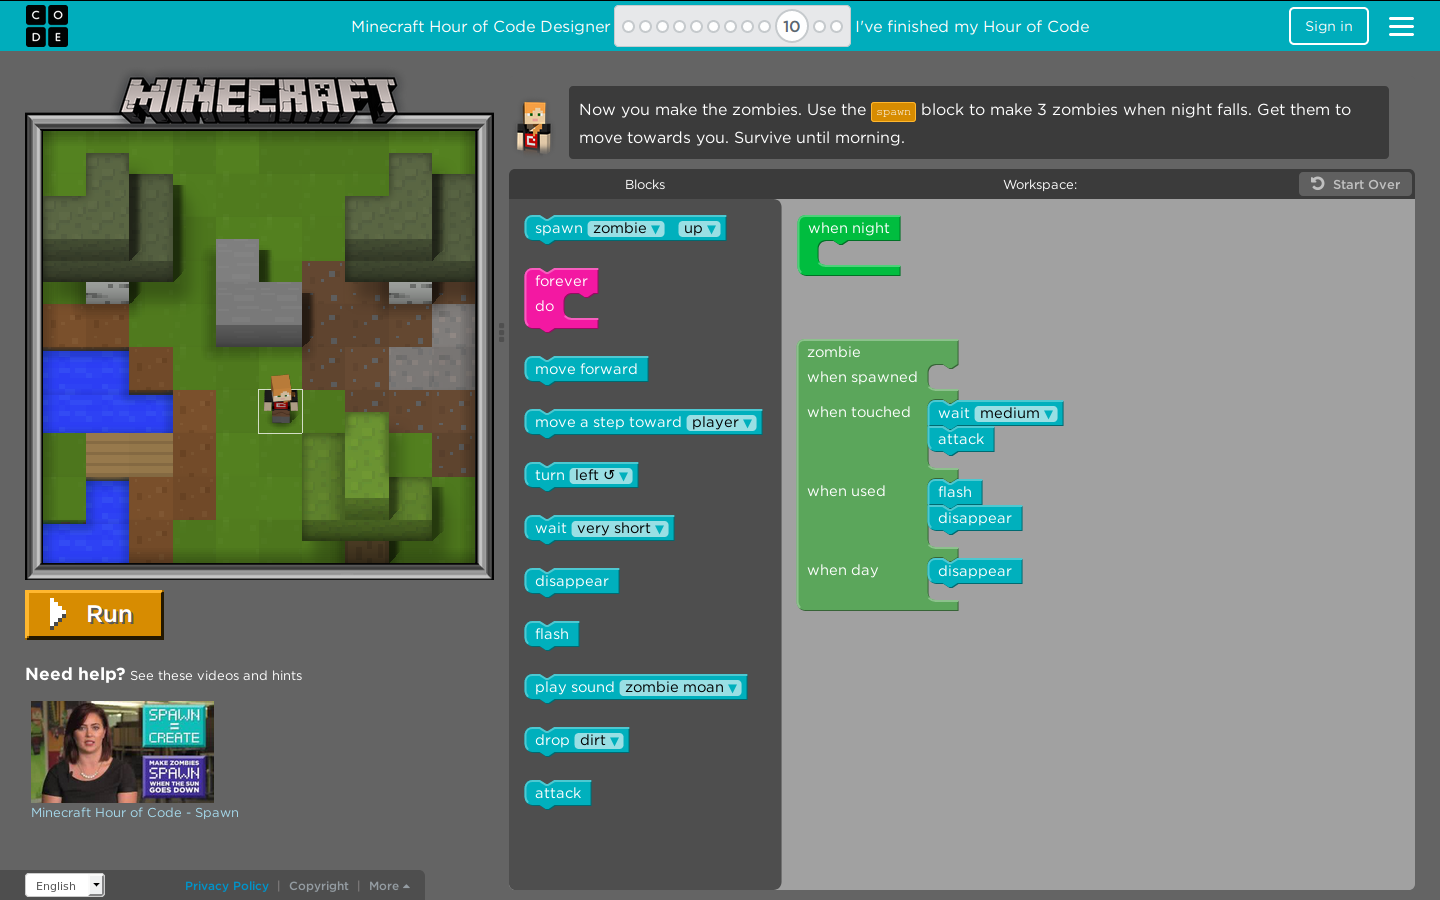
\includegraphics[width=15cm]{Images/HourOfCode.png}\par
}
It uses a simple block editor and to simulate code for lots of its coerces but it also offers some in known languages such as JavaScript and Python. They show you the basics and then give you a sand box to let you show off your programming skills.

What can I take from this?:\newline
Selling the product as a game but actual just teaching programming looks like it is quite a good way to get people to pick up the basics of coding but if I want to retain my audience so I can teach them the advanced programming slowly I need some engaging content that keeps the player hooked.

The purely educational games I have looked at don't directly apply to my project but the way that they are set out and marketed could be very useful information to try and get my project not just functional but useful in an education to teach programming on all levels.


\newpage
\subsection{Issues and Limitations:}
The scope of project that I have set out for my self is most likely not possible in the time given but to get a functional prototype with lots of the functionality and the ability to easily add more features is probably possible in the time scale given. Also there is now a large plethora of ways to make interactive content on the internet. The classic way of doing it would be in a flash window or a Java web app but those are mostly out of use so I would have to use a HTML web canvas and JavaScript or some other web language that compiles to JavaScript to make the functionality.

\subsection{Requirements:}
After talks with some of the stake holders and 

The will try and get the project to have a flexible hardware requirements. I think that the end project will require:
\begin{itemize}
    \item A moderate computer to low end computer.
    \item Network connection to the server.
    \item A modern web browser with HTML5 and CSS.
    \item A central server for clients to connect to.
\end{itemize}

The project that I have laid out has a set of criteria to meet for me to class it as a success

Success criteria
Critical:
\begin{itemize}
    \item \textbf{Centralised server}\newline
    There will be a server that all the connections go through.
    \item \textbf{Users can connect to an account on the server}\newline
    You will be able to log-in and connect to that user's account and manage settings and user code
    \item \textbf{The user can submit and run code}\newline
    You can upload code to the server and it will run in game to control the world
    \item \textbf{A graphical display of the world around the player}\newline
    An interactive view will be in the users browser and you will be able to pan the camera around the world with the mouse or keyboard.
    \item \textbf{A central world that all the users connect to}\newline
    A world stored in one or many files that is dynamically loaded for users to interact with. Possible for multiple users to be interacting with the same section at once with out desynchronisation.
    \item \textbf{Secure code execution while player is offline}\newline
    Code that the player submits for there robots to execute will continue to execute while the player is not online and will halt safely when errors are met and will report errors to the user once they log back in.
    \item \textbf{Sand boxed code environments}\newline
    The users code will not be able to leave its scope or damage the system through functions such as os.remove() or global variables.
    \item \textbf{Simple to understand tutorial}\newline
    Easy to understand tutorials on how to use the custom instructions needed and a more in depth tutorial on how to program python for beginners to help accustom them to the game environment and programming in general.
    
\end{itemize}
Desired:
\begin{itemize}
    \item \textbf{Integrated IDE}\newline
    An IDE that the user can use to produce test and submit code in while in the online application. It should have syntax highlighting and syntax error detection and identification.
    \item \textbf{Scalable implementation of items}\newline
    A simple and scalable setup for black data and item handling allowing quick implementation of new items in to the game through a simple file setup or system, possibly JSON or some other object notation
\end{itemize}

\newpage

\section{Design}
\subsection{Game Design}
\subsubsection{Inspiration}
The game its self will borrow heavily from the mechanics of Factorio as this is a well established game but it is lacking a MMO which many users of the game say they want. The main premise of Factorio is that there are a few raw materials that you build sprawling factories to utilise. In Factorio it is Iron, Copper, Coal, and Oil. With these you have them mined, shipped on conveyor belts and processing in machines to be moved along more conveyor belts. I am just borrowing the general mechanics from the game as it has spawned an entire genera of games, all with similar mechanics. In my version of the game you will have robots instead of conveyor belts. And instead of sprawling complex trees to make materials you will instead have big factory buildings that do that for you, they just need the raw materials.

The programming sections of the game will be implemented like how Screeps\_> does it. This will be that each robot has some simple code it will go over with the ability to do abstract things automatically or programmed at a lower level.

The tutorials will be similar to how An hour of code does it. Laying out a scenario where the code can be used to show how each section works. There will also be some code documentation so it can be reffed to with out having to start the tutorial.

\subsubsection{Mechanics}
The game world will be broken in to chunks. They will most likely be about 128x128 tiles big. They will contain different amounts of resources in deposits. The key resources in the game will be Iron, Copper and Stone. It may not be accurate to real life but it will make logistics in the game a whole lot easier.

The user will be able to construct some key buildings and entities such as:

\begin{tabular}{l | l}
Item & Use \\
\hline
Power Generation & This will be used to generate Power\\
Factory Buildings & These will produce robots and items to be added to storage\\
Robots & These will run code and interact with the world\\
Storage Networks & This will allow your robots and factors to access your items\\
Misc & Such as defensive walls and paths
\end{tabular}

These are the key components in the game.

\textbf{Factory Buildings:}\newline
The Factory will be placed in a chunk and will have a goal item set. It will access the storage network and start crafting everything needed to make the goal item. It will go continually until it is out of raw materials for the production of the goal item. It will place the created items and intermediate products in the storage network for the robots and the factories to use. The factories will be in 2 distinct groups. Production factories that will make items and Robot factories that will produce robots with addons. These robots and addons will take resources from the network that will be produced in the Production factories such as lasers or engines.

\textbf{Power Generation}\newline
The robots and factories will need power. To do this you will have to construct solar or wind farms. The power will be distributed with a power distribution pylon. This will witlessly power the chunk. When there is not enough power in the network the factories will suffer a speed reduction and robot's will charge slower so will run out of power. A robot that runs out of power will just stop operation for the ticks that it does not have enough power to do that step and will wait till power is restored and continue where it left off.

\textbf{Storage Network}\newline
They way that items will be stored is in a wireless network. It will be accessible in any chunk where you have a transmitter and will be shared over chunk boundaries with networks owned by you. The network will require power to stay operational. The items can be dropped off or picked up at the cost of electricity if you are in a chunk with the broadcast antenna. To attach storage to the network you will have to place matter drives in a chunk with an antenna. If the storage is full and items are being dropped off an error will be raised. The network will be susceptible to hacking by other robots. The hack time will be dependent on the size of the network and the network can also be defended with defence computers placed in the reach of the storage network. Once a network is hacked it will stay open to the hackers robots for a few ticks. This makes defending your boarders a priority.

\textbf{Robots:}\newline
The robots will be created in Robot Factories out of the necessary recourse. Robots will have some stats linked with them that can be changed by adding modules to them such as storage or weapons. Different levels of robots will have different outfit amounts.

\begin{tabular}{l | l}
Stat & Use \\
\hline
Storage & Amount of items the robot can hold before having to deposit them. \\
Armour & Amount of armour, so how much the robot can be attacked before failing. \\
Hack & How effective the robot is at hacking into the opponents Storage  network.\\
Battery & The power the robot can store for out of chunk use. \\
Weapons & The amount of weapons space available. \\
\end{tabular}

The robots will have 2 main types of weapons they can use, melee and ranged. The melee weapons will directly attack from close up where the robots will need to be in adjacent tiles and the ranged weapons will work from anywhere in there range.

There will also be hack type weapons where you try and gain access to there robot and claim it as your own. 

For combat between the robots there will be automatic detection if the enemy is hostile. This will be done between factions. So you start unaligned to any faction so are an enemy to all. But if you make an alliance with a faction you will cannot be attacked by them. With factions added to the game this could promote co-operative play between players.

The robots will be programmed in Python. there will be a custom import to interact with the word in the game. These are the instructions I think will be necessary for interaction with the world to be easy and intuitive.

\begin{table}
{\renewcommand\arraystretch{1.25}
\begin{tabular}{l|l|l} \hline
Name & \multicolumn{2}{l}{Description} \\ \hline\hline
scan & \multicolumn{2}{p{14cm}}{This will scan the current chunk and return a dictionary of the current chunk such as minerals, robots, factories etc.} \\ \hline
mine & \multicolumn{2}{p{14cm}}{This will take a resource as an input and it will then cause the robot to navigate towards the deposit and start gathering, or you give it a co-ordinate for more direct control} \\ \hline
deposit & \multicolumn{2}{p{14cm}}{This will cause the robot to deposit its content into the storage network if it is accessible from that chunk} \\ \hline
pickup & \multicolumn{2}{p{14cm}}{Pick up materials from that chunk network} \\ \hline
info & \multicolumn{2}{p{14cm}}{You give this function grid co-ordinates and it will return the info for the tile and/or entity in a dictionary} \\ \hline
move & \multicolumn{2}{p{14cm}}{The robot will path find to the given co-ordinates in the chunk, or in the given direction.} \\ \hline
moveChunk & \multicolumn{2}{p{14cm}}{Path find to those chunk co-ordinates or to the chunk in the specified direction.} \\ \hline
attack & \multicolumn{2}{p{14cm}}{Attack in the given direction or in the direction of a given co-ordinate} \\ \hline
hack & \multicolumn{2}{p{14cm}}{This will start the robot hacking into the storage network of that tile if it is not owned by the user} \\ \hline
\end{tabular}}
\end{table}

\textbf{Error handling}\newline
For error handling I will have the modal that the user imports raise standard python Errors. such as "\code{mio.StorageError}" This would allow the user to implement error handling with a simple try/except in there code. As errors being raised my cause robots to execute code in an odd way if skipped over an uncaught error in there code will cause them to halt operation and stay still where they crashed.

\textbf{Misc Buildings}\newline
The game will also have other buildings that the user can build that will help with the operation or defence of other buildings. This will be things such as:

\begin{tabular}{l | l}
Building & Use \\
\hline
Walls & These will act as a barrier that will have to be attacked to breach. \\
Gates & These will behave similarly to walls but will allow your robots to pass. \\
Beacon & This will be a way to name a co-ordinate so robots can travel to it easily. \\
Radar & This will give you active view in the surrounding chunks. \\
Path & This will improve robot travel speed. \\
\end{tabular}

\textbf{Walls:} These will stop robots from crossing acting as a barrier. They could be set up as a perimeter to help keep attackers out of your base. They will have a high defence and will be rather cheep for production. 

\textbf{Gates:} Gates will act almost identically to walls but will be more expensive and have a lower defence. They will let your robots through and optionally allied robots.

\textbf{Beacon:} This will allow you to tell robots to path find to a location by the name or ID of the beacon. This would only work for beacons owned by you or ones you given access to. This stops you needing a unique name for every beacon in the game. Just beacons owned by you.

\textbf{Radar:} This will allow you to see into the chunks surrounding the radar. The game will only allow you to see chunks that you have access to, this stops you being able to scroll your screen to someone's base and promotes expansion of your base. View able chunks will be shared between allied users.

\textbf{Path:} Path will allow the robots to travel quicker than they usually can on natural terrain allowing you to set up transport routes between sections of your base.


\newpage\subsection{Top Down Design}

\renewcommand*\DTstylecomment{\rmfamily\color{green}\textsc}
\renewcommand*\DTstyle{\ttfamily\textcolor{black}}
\dirtree{%
.1 MIO.
    .2 Client.
        .3 Display World.
            .4 Connect to server.
            .4 Check Data.
                .5 Validate Check Sum.
            .4 Display Content.
        .3 IDE.
            .4 Input Code.
                .5 Syntax Highlighting.
                .5 Error Checking.
            .4 Send Code.
    .2 Server.
        .3 Client Management.
            .4 Log-in.
                .5 Check Password.
            .4 Manage Settings.
            .4 Make an Account.
                .5 Email Verification.
        .3 World Management.
            .4 Load World.
                .5 Open File.
                .5 Get Active Chunks.
                .5 Cast to Memory.
            .4 Run game Tick.
                .5 Find Active Chunks.
                .5 Update Active Chunks.
                    .6 Find Entities in Chunk.
                    .6 Run Code on Entities.
                    .6 Update Chunk with code Output.
            .4 Save World.
                .5 Stop Ticks.
                .5 Open File.
                .5 Save Active Chunks.
                .5 Save To File.
}
This break down is useful as it takes the program and splits it into 2 main components. The Client and the Server. These programs will be running on different computers where there will be many clients connected to the same server.
The list here is not the full decomposition but it does brake it down in to much smaller parts. The full decomposition will take place for each of the small sections.

\subsection{NetCode}
With the program relying heavily on sending information to and from the server the main backbone of the program will be the network code so this will be my initial design. I will try and work it to be expandable and adaptable. As I will need to send the data between the client and the server of different types such as a game state update or the user uploading code. I have decided to use TCP for the network protocol as it will grantee that the data will get there in the right order and if the connection drops it is handled by the transport layer so it can be caught in the program.
I could use UDP for this but I would have to implement the packet ordering my self and the catching if the user disconnects would be more difficult. But it would not have a grantee that the packet will get there with out raising an error so I would also need to implement the packet error handling.
UDP allows for faster connections with more bandwidth but as I need all the packets to get there and the tick updates for the game will not be to often I can utilise the more stable connection of TCP.

For the data that the network will transport I have decided to use JSON as my packets. I could use raw data and format the packets my self but as I am having it interpreted by multiple languages, such as the client and the server, I am going to use a standard object notation.

I think that the packets should have a standard structure

\begin{lstlisting}[language=Python, caption=JSON Packet example]
{ # Packet start
    [ # Item 1 Start
        0, # Packet ID
        00, # Protocal ID
        ["DATA"] # Packet Data
    ], # End Item 1
    
    [  # Item 2 Start
        1, # Packet ID
        01, # Protocal ID
        ["DATA"] # Packet Data
    ]
} # End Packet
\end{lstlisting}

This structure would be useful as it would let me have multiple packet types handled by the same transfer code. So I could have a different packet ID for each instruction that would need to be sent between the client and the server. With the current design I think that I could use these IDs. I have split it into blocks so you can tell what each code means and so it will be expandable it will also keep similar IDs close numerically.

\begin{tabular}{ l | l }
  \hline			
  ID & Description \\
  \hline
  \multicolumn{2}{c}{0X Block, Network and Log-in} \\
  \hline
  00 & Used for network connection and connection hand shake\\
  01 & Used for Profile management\\
  03 & Used to set up an account\\
  09 & General Error handling\\
  \hline
  \multicolumn{2}{c}{1X World and program management} \\
  \hline
  10 & This will be used to request and send world chunks to the client\\
  11 & This will send and receive code chunks from the user\\
  12 & Chunk update, only updates chunk instead of sending new one\\
  13 & Chunk specific error handling such as invalid requests or no permission\\
  \hline
  \multicolumn{2}{c}{2X Client Management} \\
  \hline
  20 & Used to send IDE tools to the user's client\\
  \hline  
\end{tabular}

This set up means that I can have an expandable network packet system. I can add more IDs if I feel that it is necessary but this should be enough to keep them separated into functional groups for easy tracking and debugging of the code once I start to set it up. 
With the ID blocks set up this will make it easy for the World Management and Client Management sections of the server to hand off the instruction to the sub functions by checking the Protocol ID.

The main server can just read the ID block and then delegate the packet to the necessary section of code. This will keep the code clean and manageable.


\subsection{Function Descriptions}
\subsubsection{Server}
By far the largest part of the code will be the server. It is responsible for keeping all the users synchronised to the serve and the connections alive. It also handles the word being run each tick.

The 2 main parts of the server are world and client management. Client management will be responsible for keeping the user accounts secure and managing the settings that the user chooses.

\textbf{Client Management}\newline
\textbf{Log-in}\newline
The first part of this will be to log them in. For this to start the server will have a socket opened by the client to the server. It will send a data packet requesting to connect to the server. This will use protocol 00. The server will respond saying that it has accepted the connection and tell the client what it needs, [E-Mail and Password]. This will be sent via a secure socket. The E-Mail will be searched through the database and then the password will be hashed and salted and compared to the data base. The hash and salt method of password verification will mean I don't have to hold passwords on the server. Just strings. First I would take the salt in the database and add it to the string. I would then put it through a one way function known as a hash. Theses already exist so I would just import the function. If the user has a valid password I will generate a key for them to use for verification on this session.

The session key will be linked with there IP address that I will have gotten from the socket when it opened. So for there communications with the server they can use the key to authorise access to there account instead of there password for every action. They key will be invalidated when they log off. And will be linked with there IP to stop people using the key if they are not who they say they are.

The session key will be sent to the user over protocol 00 and the server will request that the client sends the key back just to verify that it is in the database correctly.
When the connection is verified the client will have to request the next section of operation such as world requests or changing settings.

To keep them connected the key, IP and userID will be saved to the database. This means that when they request access I can verify the information on the fly with out having to log back in. It will be removed from the database when it is invalidated.

This should hopefully keep the user's account secure while letting them use it with out having to constantly log-in in again. Although with there IP being linked with the key they will be denied access when there IP changes. This could be a problem if it is used on a mobile network as they can change IPs quite frequently

\textbf{Manage settings}\newline
This will be much simpler than the log-in as all of the user verification is done. This section of code will take a key, check the IP and then get the information for that user from the data base. Such as IDE settings, password and UserName. This will all start when a request is made by the user over protocol 01. When the user has the current information they can request a change, again with protocol 01 and if the key and IP are correct the database will be updated. If the E-Mail is changed it will have to be re-verified. The verification process will be the same function used in setting up the account. (This will be described in that function.)

\textbf{Setting Up and Account}\newline
This will be similar to loggin in where the client open a socket. But it will start the connection over protocol 03. The server will respond and ask for a UserName, E-Mail, and password. The password will be checked client side. So the client window will have them type the password in twice to verify that they did indeed type what they wanted. I will restrict the password to be more than 8 characters and have characters from 2 at least 2 character sets such as Uppercase, Lowercase, Number, Special, and Other. The other section will include the rest of Unicode. This may make it more difficult to make a password in a language with out Latin characters but as the game will only be offered in English I am not keeping this as a concern.

When this info is received the account information will be kept in a database table for pending users and an E-Mail will be sent to them with a code.
\begin{figure}
\begin{mdframed}
\makebox[\textwidth]{Verification E-Mail} \par
\noindent\rule{15cm}{0.4pt}
From:\par
\framebox[10cm]{verification@example.com}\newline
Subject:\par
\framebox[10cm]{MIO Email Verification} \par
To:\par
\framebox[10cm]{user@example.com}
\newline
\noindent\rule{15cm}{0.4pt}
\newline
Welcome to MIO, the Python Programming MMO. Here is your verification code:\newline
\framebox[1.1\width]{cmFuZG9tIG}

\end{mdframed}
\caption{Mock Up Verification E-Mail}
\end{figure}

This will give the user 10 digits of random Base64 string. This will be saved with the pending user. The user will be able to input this now while setting up the account where it will be checked. If it is they will be moved to the main user database and will be able to play the game. If they lose connection or close the window they won't be able to enter the code here so when they next log-in with protocol 00 it will find that the user is not in the database so it will check the pending users if they are a pending user it will ask for the verification code. When the user has finally verified them selves with the code they will be moved to the main user database and have default settings established, these can be changed later. After the user account is set up they will go through the normal log-in procedure


\textbf{World Management}\newline

The server is also responsible for keeping the world active, keeping the robots working in the chunks, displaying the world to the user, and updating the world when it ticks.

In the world I am going to quantize time so have every robot run through its code every tick. This will be the unit of time in the game. So after each tick the client will get an update file with new positions of the robots and items in the chunks they currently have open. The problem with having the robots go through the code every tick is that some robots may have gotten stuck in a loop so would not have a finite time complexity that can be resolved in the short amount of time. I will find solutions to this when going through the game tick in more detail.

\textbf{Load World}\newline
A key part to the game is having a large world where all the users interact. For this the world needs to be able to be split in to small chunks and saved to persistent storage. I will be utilising a directory tree to have the world split up into chunks. Each chunk will have a main file that will define the area and a folder that will have information on active entities in the chunk such as robots. The chunks will be named by the 2D co-ordinate system that I will be using internally. This will mean that I can call a chunk by its co-ordinates so I can easily find the needed information to give to the user.
I won't use any leading 0's on the chunk name as this will limit the number of chunks I can use. And I will leave it in base 10 as this is easy to understand and compute with.
\newpage
\dirtree{%
.1 /.
    .2 code/.
        .3 CODE FILES HERE.
    .2 userData/.
        .3 HKbaG6dBC1dVxMLLDOqFoQ.json.
        .3 HKbaG6dBC1dVxMLLDOqFoQ/.
            .4 code/.
        .3 KN7Ec9h8hhwtBX\_flTvP7w.json.
        .3 KN7Ec9h8hhwtBX\_flTvP7w/.
            .4 code/.
        .3 5DyGnHW7wmC97rrOzgO9SA.json.
        .3 5DyGnHW7wmC97rrOzgO9SA/.
            .4 code/.
    .2 world/.
        .3 active\_chunks.csv.
        .3 0x0.cnk.
        .3 0x0/.
            .4 robot\_xckH7qFDXDc9lAjVsGlCeA.json.
            .4 robot\_1M9ZM20G204zYRdU8q-rlw.json.
            .4 robot\_l1FsJ1cI65pG6LcIiVwFug.json.
            .4 facto\_6bX3BYTV6wwyOmdLyrwdHg.json.
        .3 1x0.cnk.
        .3 1x1/.
            .4 robot\_f7\_Wnc130qybYW4O5Jc2Vw.json.
            .4 facto\_i481qfIwq71j2rSoxbLA5w.json.
}

The long sections of random text such as "HKbaG6dBC1dVxMLLDOqFoQ" are 16 characters for a base64 string. I am going to use this as an ID as it is fixed length, random and easy to use. The users JSON file will have an array for linked robot and facto files. This way they can find the information they need. I could use a relational database for this but I am going to implement a relational manager in the code to keep the references valid and this way I can have a many to one relation with out having the user ID with the robot as this will take longer to search through. With the IDs being with the user file they can find all linked items quickly with out scanning the whole database. JSON format is also easier to work with in Python and JavaScript. This will save the overhead of having a DBMS running in tandem with the server. 

To begin to load the world the program will first open active\_chunks.csv. This file will contain a list of chunks with currently active entities in them. These are the chunks that need to be in ram and have a game tick run on them. The file will just be a list of the chunks with active tiles in them separated by commas. The programme will go through the list and add the active chunk to the list in ram. This will be quicker to run over than the file in permanent storage. This is the main part of the world loading program as the world exists in permanent storage and chunks will be dynamical cast to ram when requested.

\textbf{Run Game Tick}\newline
This is by far one of the largest sections of code that will be used. It is the code responsible for running all the actions in the game. This section need further functional decomposition as it is the heart of the game code.
\dirtree{%
.1 Run Game Tick.
    .2 Run Power Tick.
        .3 Add power to the network.
    .2 Run Factory Tick.
        .3 Check if enough power.
        .3 If crafting step craft time.
        .3 Else Start craft to goal.
            .4 Make Dependency tree.
            .4 Check storage for completed items in tree.
            .4 Start crafting items lowest in tree.
                .5 Remove needed items from storage.
                    .6 if missing items move up tree and try again.
    .2 Run Robot Tick.
        .3 Charge battery.
        .3 Check if enough power.
        .3 Run code.
            .4 Run logic in code.
            .4 Run MIO Functions in code.
                .5 If movement needed.
                    .6 Path find to location and start movement.
                .5 If storage needed.
                    .6 Check for network.
                    .6 Use network.
                .5 If attack.
                    .6 Check for targets.
                .5 If Scan.
                    .6 Return Information.
                .5 If mine.
                    .6 extract items.
                    .6 Add to inventory.
    .2 Wait till end of time step.
    .2 Kill all code that has not finished executing at time step.
        .3 Raise Error in robots.
}

\textbf{Run Power Tick:}\newline
This step will be easy enough. The logic will be like this.

\begin{lstlisting}[language=Python, caption=Run Power Tick Logic]
for each power network:
    current_power = 0
    for each power_station in network:
        current_power += power_station.output
\end{lstlisting}
This will set the available power in the network for that game tick. It will be utilised by factories and robots to complete operations.

\textbf{Run Factory Tick:}\newline
This section of the algorithm will have to construct item trees at each step of construction to finish its product. The recipes that can be crafted will be stored as a dictionary so it can be searched via keys to find the ingredients for each product.
\begin{lstlisting}[language=Python, caption=Run Factory Tick]
# Define recursive tree function
def get_item_tree(goal, craft_tree):
    # This will give an array of the items needed to craft this
    needed_items = mio.recipes[goal]["needed"]
    
    # Check if base component
    if needed_item == goal:
        item = needed_item
        if item in network.storage.items:
            self.inventory.add(item)
            network.storage.remove(item)
            craft_tree.append(item)
        else:
            # Missing base components so can't continue
            raise mio.MissingIngredientsError
    
    else:
        for item in needed_items:
            if item in network.storage.items:
                self.inventory.add(item)
                network.storage.remove(item)
            else:
                craft_tree.append(item)
                craft_tree = get_item_tree(item, craft_tree)
    
    return craft_tree

# Check for power
if current_power >= needed_power:
    current_power -= needed_power
    
    # If crafting do craft step
    if crafting:
        time_needed -= craft_speed
        # If done crafting
        if time_needed <= 0:
            # Use up needed items
            for item in mio.recipes[crafted_item]["needed"]:
                self.inventory.remove(item)
                
            # If final product
            if len(craft_tree) = 0:
                network.storage.add(crafted_item)
            else:
                self.inventory.add(crafted_item)
            crafting = False
            
    else:
        if craft_tree == []:
            craft_tree = get_item_tree(goal_item, [])
            
        # Used depth first search of craft tree so start crafting from base of tree.
        crafted_item = craft_tree[-1] 
        del craft_tree[-1]
        time_needed = mio.recipes[crafted_item]["time"]
        crafting = True
            
        
else:
    raise.mio.NoPowerError
\end{lstlisting}

The function to generate the crafting tree utilises a recursive depth first. This means that I can work back up the tree with confidence that all the needed items are already in the inventory of the factory. This approach will decompose every thing to the minimum item that is in storage or to the raw components. If any raw components are missing then the crafting will not start as a full claimed tree can not be produced.
Items are claimed into the factories inventory so they can't be used by other factories while the item is crafting.
The factory will also need to be able to cancel any crafting if the player wishes to change anything. This would cause the factory to dump it's inventory into the storage network and clear its own inventory. This will leave the factory in a state where it can make a new tree and start crafting again.

To test the code I can run it with a set of ingredients in the storage network and give it some recipes to try and craft with the ingredients. 

\textbf{Run Robot Tick:}
This will run the code in the robot in the time frame given. The robots will be given a limited amount of time to run the user submitted code as this will stop them getting stuck in an infinite loop and halting the server.
Each robot will run in a thread so they can all execute concurrently. To test the robots I will construct code in the robots language with expected outcomes and test it. The robots will use raw python code that will be run with the \code{exec()} The exec function can be quite dangerous for giving users input as they can use built in functions to destroy the server. But you can limit the name space of the execution. This way I can only give them known safe functions. I can even rename functions for the name space. So when they call \code{print()} it can instead call a function that prints to the user not the server terminal.

With the limited name space I can give the user full access to python. This will make it easy to run the user code.

The robots will be able to access the modules that I give them. The module includes functions that will move the robot around the world automatically to different co-ordinates. This will require a pathfindeing algorithm to let them get around quickly. I have derided to use the A* search algorithm as it allows me to use holistic to reduce the time complexity of the solution. It will give sub optimal solutions but this is fine as with the timed conditions for the large number of time it will run.

The mine function will interact with the world and remove items from the location below and place it in the invetory of the robot.

The checking for storage will just be a call to the storage network object. This will return items, errors or other such things if needed.

The scan function will just request chunk data from the current chunk and save that as a dictionary for easy use.
\begin{lstlisting}[language=Python, caption=Chunk scan return]
{
    "factories":[
    # List of factories
    ]
    "resources":[
    # List of resources with attacked locations
    ]
    "robots":[
    # List of robots with ID, Owner, and position
    ]
    "network":[
        "storage": # Owner and network info
        "power":   # Owner and network info
    ]
}
\end{lstlisting}


\subsubsection{Client}
The client is what the user will be using to connect to the server. The client will be a web page that will be viewed from a browser.
There will be 5 main sections to the site. An introduction page, A log-in page, A settings page, the game window, and the code Documents

The first part of the server is to establish a connection to the server. The browser will handle the main part with a https request. That way I can serve the site to the user. But for more server interactive sections such as the game, log-in, and account management it will be done via JavaScript and web sockets. This will allow me to talk to the server while leaving the page responsive to the user.

\textbf{Main Page}\newline
The main page will have a navigation bar allowing you to access the rest of the site and a introduction to the game. 

{\centering
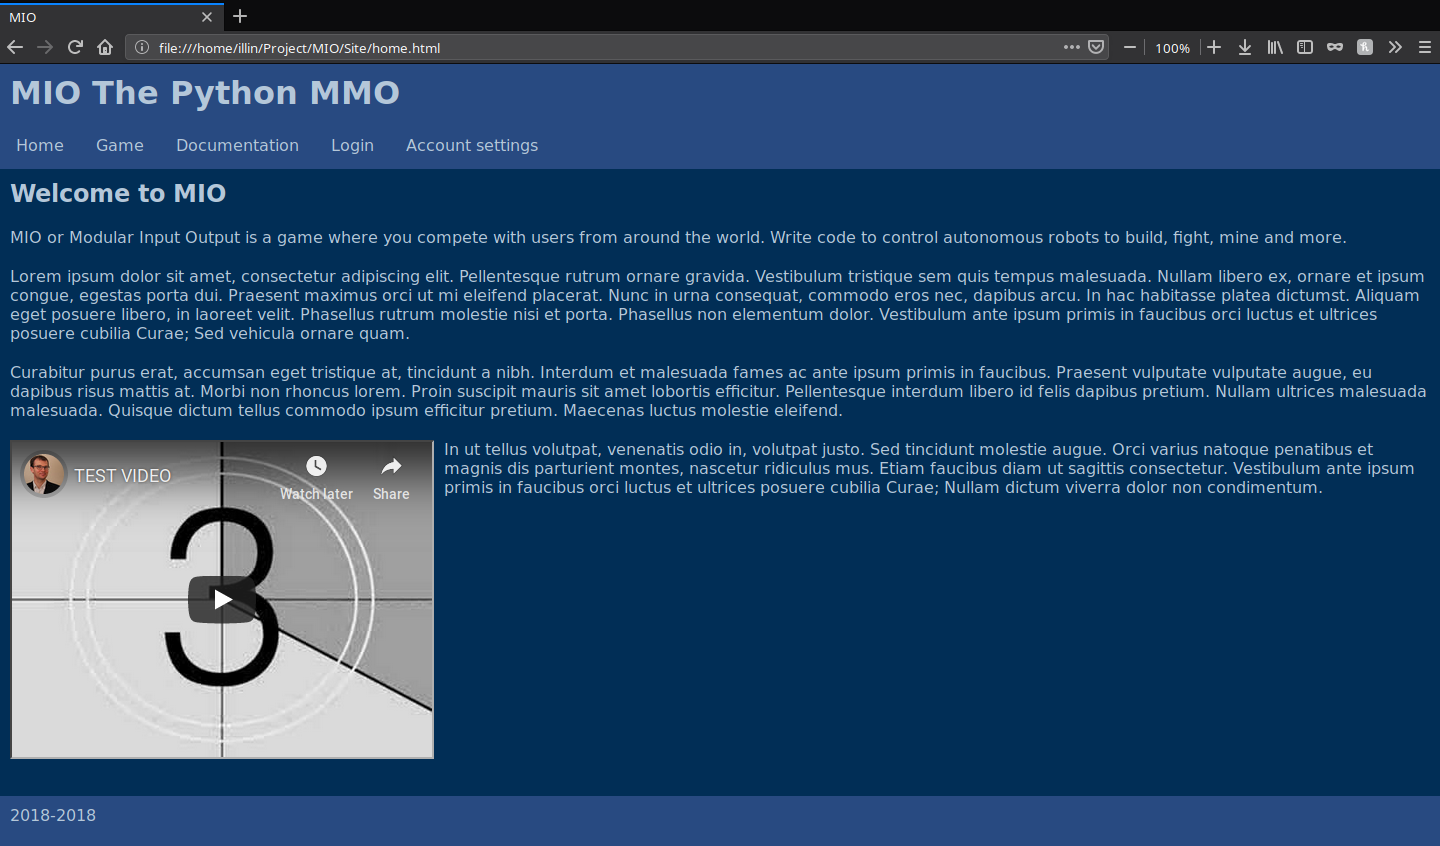
\includegraphics[width=15cm]{Images/Design/homepage.png}\par
}

The page will be mainly text and possibly an introductory video to the project. This is unlikely though. The main section of the game's site will be an advertisement for the game and a short introduction to how the game works.

\textbf{Log-in Page}\newline
The log-in page will provide a simple screen for logging-in to your account. It will have a box to enter E-Mail address and your password. With a sign up button for new users. If any of the information given is wrong the client won't be told if the ether the E-Mail or Password is correct for security purposes and it will say \code{The log-in credentials are incorrect}

TODO [INCLUDE MOCK UP SCREEN SHOT]

\textbf{Code Documentation}\newline
For the code documentation part of the site I will not use my own server as there are many standards that are best to keep to when documenting the code. For this I will use the website \code{www.readthedocs.org} This site hosts the documentation in an easy to use format that is intuitive and used all ready by many professional projects such as the BBC Micro:Bit

The documentation will be set up in reStructuredText format. This makes it easy to search through and easy to write documentation. It supports inline code snippets so I can provide code examples for the users to try out.

\textbf{Game Page}
The game page will be a blank page with a JavaScript webcanvas. It will allow the user to interact with the game world in the browser.

The game will be made up of 2 main screen types. A world view and a code view. The world view will let you view and interact with the world in the game, it will let you modify settings in buildings and in robots.

\begin{tabular}{| l | l |}
\hline
View of the world \hspace{6cm} & Building/Robot information\hspace*{0.5cm}\\
&\\
&\\
&\\
&\\
&\\
&\\
&\\
&\\
&\\
&\\
\hline
\multicolumn{2}{|c|}{General chunk information or Code snippets (Collapsible)} \\
\multicolumn{2}{|c|}{} \\
\multicolumn{2}{|c|}{} \\
\multicolumn{2}{|c|}{} \\
\hline
\end{tabular}\\

This will be the screen layout of the world view mode. The lower section of the screen will be collapsible giving you more room to see the world and more room for information on the right hand side.
The right hand side will give current settings in the object and the code being run on the robots. With a terminal for manual code execution on the robot.
The world view section will show you the placement of the objects in the chunk with the ability to zoom and pan around the chunk and move to view other chunks.
The lower section will be able to show you snippets of the currently running code on your robot or current crafting information of your factories. It will also be able to display information on the storage network if a storage related item is selected. It will be the main way to see the inner workings of your programme setup in the game.

The game will also have a programming mode that will give you an IDE to develop code in your project.
The layout will be like this:


\begin{tabular}{| l | l |}
\hline
Files/Documents & Code Editor\hspace*{9.5cm}\\
&\\
&\\
&\\
&\\
&\\
&\\
&\\
&\\
&\\
&\\
&\\
\hline
\multicolumn{2}{|c|}{Terminal for code} \\
\multicolumn{2}{|c|}{} \\
\multicolumn{2}{|c|}{} \\
\multicolumn{2}{|c|}{} \\
\multicolumn{2}{|c|}{} \\
\hline
\end{tabular}\\

\newpage
\section{Development}
The development will follow a structure with testing after each section. The sections will all be separated into modals that can all be run and tested separately. This will allow me to check the functionality of them and debug it more easily. The order that I will be developing in will be as follows:
\dirtree{%
.1 Generic Functions and Classes.
    .2 Queue implementation.
    .2 JSON file manager.
.1 Net Code.
    .2 Make connection.
    .2 Send/Receive data at the same time.
}
\subsection{Generic Functions and Classes}
The file structure of the server will be:
\dirtree{%
.1 /.
    .2 main.py.
    .2 classes/.
        .3 \_\_init\_\_.py.
        .3 CLASS FILES GO HERE.
}
this will mean that I can have all the functions outside of the main chunk of code and have testes run separately from the classes. I will bring the classes into main.py with \code{import classes.file.class}. This will bring the class into the scope of the current file.

\subsubsection{Queue:}
The first part is the queue. The queue will handle an array that can have items put on to the queue at the end and will have data taken from the top of the queue. This will be useful for making sure the order of instructions executed by the server will stay in order. If they are all in a queue then they will have a coherent order and be executed in the order that they arrive.

The queue was fairly easy to code as there are standard practices for setting up a queue. Here is my implementation:

\begin{lstlisting}[language=Python, caption=Python Server Test]
# Implementation of a queue
class queue:
    def __init__(self):
        self.queue = []

    # Dequeue from list, return None if no data
    def dequeue(self):
        if len(self.queue) > 0:
            data = self.queue[0]
            del self.queue[0]
            return data
        else:
            return None
    
    # Add data to the que
    def enqueue(self,data):
        self.queue.append(data)

    # Return length of queue
    def len(self):
        return len(self.queue)

    # Return true if queue has data
    def isdata(self):
        return self.len() != 0
\end{lstlisting}

The queue should be able to start with an empty queue, add data to the queue, return data from the queue and return a known item if it is dequeueing from and empty queue, in this case \code{None}

My test flow for this will be as follows:
\begin{itemize}
    \item Make new Queue
    \item Check Queue length 0
    \item Check is Data == False
    \item Add "test" to queue
    \item Check Length of queue is 1
    \item is Data == True
    \item Dequeue data, check data
    \item Dequeue and check for Null
\end{itemize}

For this project I have decided to use unit testing so I can have a program automatically test the functionality of the code and make sure it acts as expected. I have made file that runs the 8 tests and tells me if it passes or not. Here is the test for the Queue

\begin{lstlisting}[language=Python, caption=Python Server Test]
# Queue Test
print("----QUEUE TEST----")
pass_count = 0
fail_count = 0
import classes.queue
print()
print("MAKE QUEUE: \t\t",end = "")
try:
    # Testing if you can make queue
    que = classes.queue.queue()
    print("PASS")
    pass_count += 1

    # Testing if origonal length is 0
    print("QUEUE LENGTH NEW: \t",end = "")
    if que.len() == 0:
        print("PASS")
        pass_count += 1
    else:
        print("FAIL")
        fail_count += 1

    # No data should be present and queue initialisation
    print("QUEUE DATA NEW: \t",end = "")
    if not que.isdata():
        print("PASS")
        pass_count += 1
    else:
        print("FAIL")
        fail_count += 1

    # Test Enqueue data
    print("QUEUE ENQUE: \t\t",end = "")
    que.enqueue("test")
    print("PASS")
    pass_count += 1

    # Testing if origonal length is 1 after enqueue
    print("QUEUE LENGTH DATA: \t",end = "")
    if que.len() == 1:
        print("PASS")
        pass_count += 1
    else:
        print("FAIL")
        fail_count += 1

    # Should have data now
    print("QUEUE DATA: \t\t",end = "")
    if que.isdata():
        print("PASS")
        pass_count += 1
    else:
        print("FAIL")
        fail_count += 1

    # Test Dequeue
    print("QUEUE DEQUE DATA: \t",end = "")
    if que.dequeue() == "test":
        print("PASS")
        pass_count += 1
    else:
        print("FAIL")
        fail_count += 1

    # Test Dequeue
    print("QUEUE DEQUE NULL: \t",end = "")
    if que.dequeue() == None:
        print("PASS")
        pass_count += 1
    else:
        print("FAIL")
        fail_count += 1
except Exception as e:
    print("FAIL: " + str(e))
    fail_count += 1
print(f"PASS COUNT: \t\t{pass_count}")
print(f"FAIL COUNT: \t\t{fail_count}")
print("------------")
\end{lstlisting}
The error handling in the test code is bad. This is because if the test does raise an error then I want it to just print fail and end the test. So I have placed all the tests in a try statement. The output of the code is as follows:
\code{
----QUEUE TEST----\\
\\
MAKE QUEUE:             PASS\\
QUEUE LENGTH NEW:       PASS\\
QUEUE DATA NEW:         PASS\\
QUEUE ENQUE:            PASS\\
QUEUE LENGTH DATA:      PASS\\
QUEUE DATA:             PASS\\
QUEUE DEQUE DATA:       PASS\\
QUEUE DEQUE NULL:       PASS\\
PASS COUNT:             8\\
FAIL COUNT:             0\\
------------}\\
This is good as the queue has passed all tests that were layed out for it. Now I can move on to the next section of code. The JSON file handler.

\subsubsection{JSON file handler}
This code will be used to manage JSON files on the disk. It will be used for things such as settings and chunk data. 


\subsection{Net-code}
The first large section in the net code. I will start with a basic python program that can talk to a JavaScript client. This will let me start on the main part of the game. The success criteria for this is the success full asynchronous transition of strings between the client and server. It will be tested by having the client send information to the server and the server echoing it back. Then the server will send a message this will make sure that the client is not blocking transition or reception. The client will then send two messages and if all message got through in the right order than the code will success.
\begin{itemize}
    \item Client Send string to server.
    \item Verify message and echo back.
    \item Server sends second consecutive message.
    \item client sends two consecutive messages.
\end{itemize}

The code will have a Python server and a JavaScript client running in Firefox for current testing. I will be using the python web sockets modal as it handles setting up the socket leaving all the logic to me. It also provides a means of signing the socket to make it secure at a later date.

My first test was setting up the bare bones send and responce before setting up the asyncronous communication:

\begin{lstlisting}[language=Python, caption=Python Server Test]
# Sol Steele
# Initial server test

import asyncio  # Handles asynchronous input output
import websockets  # Handles webosocket connections

async def run_socket(ws, path):
    print("Connection")
    # Wait for blocking function to get data from socket.
    name = await ws.recv()
    print(name)

    # respond with greeting
    await ws.send("Hello " + name)
    print("Connection Closed")

# Name function to start server
start_server = websockets.serve(run_socket, 'localhost', 5678)

print("Start")
# Define main loop
asyncio.get_event_loop().run_until_complete(start_server)
print("Enter Loop")
asyncio.get_event_loop().run_forever()

\end{lstlisting}

\begin{lstlisting}[language=JavaScript, caption=JavaScript Client Test]
// Define The Socket Object
var ws = new WebSocket("ws://127.0.0.1:5678/"),
    name = window.prompt("enter name","");
// Send the name to the server through the socket
ws.send(name)
// Event holds the page untill  message is recived
ws.onmessage = function (event) {
    alert(event.data)
};
\end{lstlisting}

This code can successfully transmit a sting to and from the client and the server. The next step is asynchronous data transfer so that they can communicate and handle blocking functions. For this I will create functions that listen and send from a queue and separate threads. This will allow the main thread to run with out needing to wait for a message to be found or sent.

To achieve the simultaneous input and output of data I will be using a queue for incoming data from the client. I have implemented a queue as a class object.
\begin{lstlisting}[language=Python, caption=Queue Class]
# Implementation of a queue
class queue:
    def __init__(self):
        self.queue = []

    # Dequeue from list, return None if no data
    def dequeue(self):
        if len(self.queue) > 0:
            data = self.queue[0]
            del self.queue[0]
            return data
        else:
            return None
    
    # Add data to the que
    def enqueue(self,data):
        self.queue.append(data)

    # Return length of queue
    def len(self):
        return len(self.queue)

    # Return true if queue has data
    def isdata(self):
        return self.len() != 0
\end{lstlisting}
After many attempts to get the code working using the websockets modual in python I have failed to get it working.

\end{document}
